% Created by tikzDevice version 0.12.6 on 2026-05-17 11:03:54
% !TEX encoding = UTF-8 Unicode
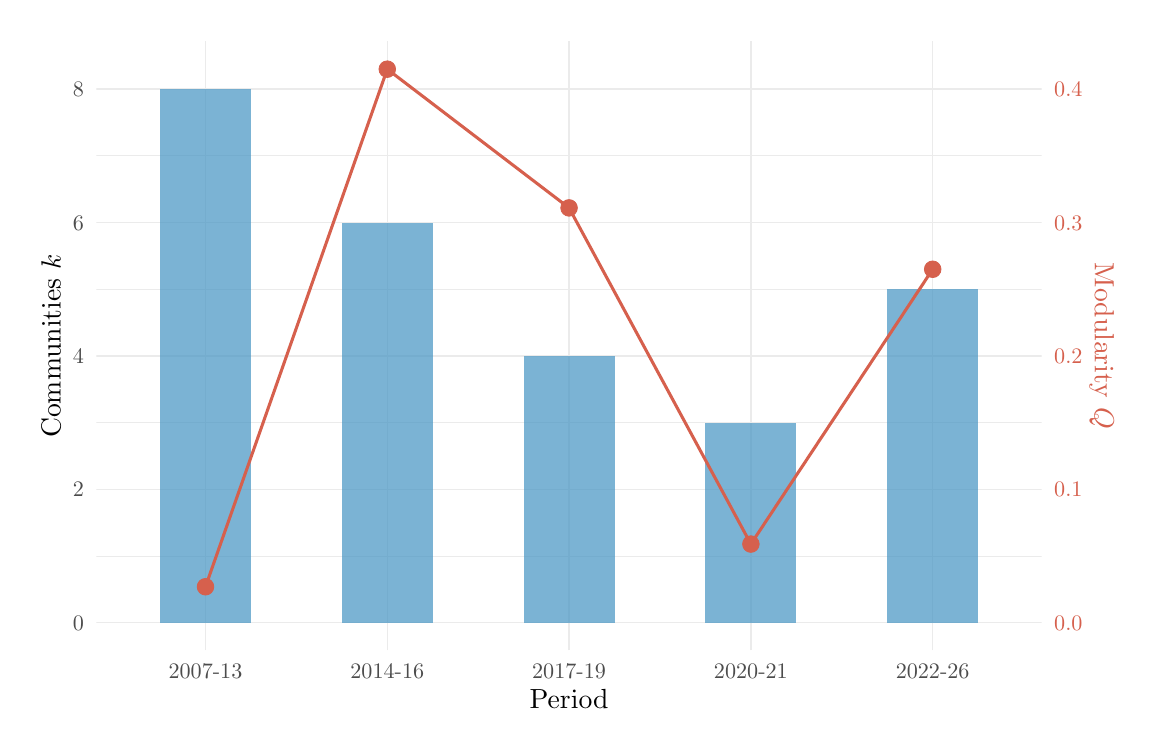
\begin{tikzpicture}[x=1pt,y=1pt]
\definecolor{fillColor}{RGB}{255,255,255}
\path[use as bounding box,fill=fillColor,fill opacity=0.00] (0,0) rectangle (397.48,252.94);
\begin{scope}
\path[clip] (  0.00,  0.00) rectangle (397.48,252.94);
\definecolor{fillColor}{RGB}{255,255,255}

\path[fill=fillColor] ( -0.00,  0.00) rectangle (397.48,252.94);
\end{scope}
\begin{scope}
\path[clip] ( 24.83, 27.90) rectangle (366.43,247.95);
\definecolor{drawColor}{gray}{0.92}

\path[draw=drawColor,line width= 0.3pt,line join=round] ( 24.83, 62.00) --
	(366.43, 62.00);

\path[draw=drawColor,line width= 0.3pt,line join=round] ( 24.83,110.20) --
	(366.43,110.20);

\path[draw=drawColor,line width= 0.3pt,line join=round] ( 24.83,158.41) --
	(366.43,158.41);

\path[draw=drawColor,line width= 0.3pt,line join=round] ( 24.83,206.61) --
	(366.43,206.61);

\path[draw=drawColor,line width= 0.5pt,line join=round] ( 24.83, 37.90) --
	(366.43, 37.90);

\path[draw=drawColor,line width= 0.5pt,line join=round] ( 24.83, 86.10) --
	(366.43, 86.10);

\path[draw=drawColor,line width= 0.5pt,line join=round] ( 24.83,134.31) --
	(366.43,134.31);

\path[draw=drawColor,line width= 0.5pt,line join=round] ( 24.83,182.51) --
	(366.43,182.51);

\path[draw=drawColor,line width= 0.5pt,line join=round] ( 24.83,230.71) --
	(366.43,230.71);

\path[draw=drawColor,line width= 0.5pt,line join=round] ( 64.25, 27.90) --
	( 64.25,247.95);

\path[draw=drawColor,line width= 0.5pt,line join=round] (129.94, 27.90) --
	(129.94,247.95);

\path[draw=drawColor,line width= 0.5pt,line join=round] (195.63, 27.90) --
	(195.63,247.95);

\path[draw=drawColor,line width= 0.5pt,line join=round] (261.33, 27.90) --
	(261.33,247.95);

\path[draw=drawColor,line width= 0.5pt,line join=round] (327.02, 27.90) --
	(327.02,247.95);
\definecolor{fillColor}{RGB}{67,147,195}

\path[fill=fillColor,fill opacity=0.70] ( 47.82, 37.90) rectangle ( 80.67,230.71);

\path[fill=fillColor,fill opacity=0.70] (113.52, 37.90) rectangle (146.36,182.51);

\path[fill=fillColor,fill opacity=0.70] (179.21, 37.90) rectangle (212.06,134.31);

\path[fill=fillColor,fill opacity=0.70] (244.90, 37.90) rectangle (277.75,110.20);

\path[fill=fillColor,fill opacity=0.70] (310.59, 37.90) rectangle (343.44,158.41);
\definecolor{drawColor}{RGB}{214,96,77}

\path[draw=drawColor,line width= 1.1pt,line join=round] ( 64.25, 50.91) --
	(129.94,237.94) --
	(195.63,187.81) --
	(261.33, 66.34) --
	(327.02,165.64);
\definecolor{fillColor}{RGB}{214,96,77}

\path[draw=drawColor,line width= 0.3pt,line join=round,line cap=round,fill=fillColor] ( 64.25, 50.91) circle (  3.00);

\path[draw=drawColor,line width= 0.3pt,line join=round,line cap=round,fill=fillColor] (129.94,237.94) circle (  3.00);

\path[draw=drawColor,line width= 0.3pt,line join=round,line cap=round,fill=fillColor] (195.63,187.81) circle (  3.00);

\path[draw=drawColor,line width= 0.3pt,line join=round,line cap=round,fill=fillColor] (261.33, 66.34) circle (  3.00);

\path[draw=drawColor,line width= 0.3pt,line join=round,line cap=round,fill=fillColor] (327.02,165.64) circle (  3.00);
\end{scope}
\begin{scope}
\path[clip] (  0.00,  0.00) rectangle (397.48,252.94);
\definecolor{drawColor}{gray}{0.30}

\node[text=drawColor,anchor=base east,inner sep=0pt, outer sep=0pt, scale=  0.80] at ( 20.33, 35.14) {0};

\node[text=drawColor,anchor=base east,inner sep=0pt, outer sep=0pt, scale=  0.80] at ( 20.33, 83.35) {2};

\node[text=drawColor,anchor=base east,inner sep=0pt, outer sep=0pt, scale=  0.80] at ( 20.33,131.55) {4};

\node[text=drawColor,anchor=base east,inner sep=0pt, outer sep=0pt, scale=  0.80] at ( 20.33,179.75) {6};

\node[text=drawColor,anchor=base east,inner sep=0pt, outer sep=0pt, scale=  0.80] at ( 20.33,227.96) {8};
\end{scope}
\begin{scope}
\path[clip] (  0.00,  0.00) rectangle (397.48,252.94);
\definecolor{drawColor}{RGB}{214,96,77}

\node[text=drawColor,anchor=base east,inner sep=0pt, outer sep=0pt, scale=  0.80] at (381.15, 35.14) {0.0};

\node[text=drawColor,anchor=base east,inner sep=0pt, outer sep=0pt, scale=  0.80] at (381.15, 83.35) {0.1};

\node[text=drawColor,anchor=base east,inner sep=0pt, outer sep=0pt, scale=  0.80] at (381.15,131.55) {0.2};

\node[text=drawColor,anchor=base east,inner sep=0pt, outer sep=0pt, scale=  0.80] at (381.15,179.75) {0.3};

\node[text=drawColor,anchor=base east,inner sep=0pt, outer sep=0pt, scale=  0.80] at (381.15,227.96) {0.4};
\end{scope}
\begin{scope}
\path[clip] (  0.00,  0.00) rectangle (397.48,252.94);
\definecolor{drawColor}{gray}{0.30}

\node[text=drawColor,anchor=base,inner sep=0pt, outer sep=0pt, scale=  0.80] at ( 64.25, 17.89) {2007-13};

\node[text=drawColor,anchor=base,inner sep=0pt, outer sep=0pt, scale=  0.80] at (129.94, 17.89) {2014-16};

\node[text=drawColor,anchor=base,inner sep=0pt, outer sep=0pt, scale=  0.80] at (195.63, 17.89) {2017-19};

\node[text=drawColor,anchor=base,inner sep=0pt, outer sep=0pt, scale=  0.80] at (261.33, 17.89) {2020-21};

\node[text=drawColor,anchor=base,inner sep=0pt, outer sep=0pt, scale=  0.80] at (327.02, 17.89) {2022-26};
\end{scope}
\begin{scope}
\path[clip] (  0.00,  0.00) rectangle (397.48,252.94);
\definecolor{drawColor}{RGB}{0,0,0}

\node[text=drawColor,anchor=base,inner sep=0pt, outer sep=0pt, scale=  1.00] at (195.63,  6.94) {Period};
\end{scope}
\begin{scope}
\path[clip] (  0.00,  0.00) rectangle (397.48,252.94);
\definecolor{drawColor}{RGB}{0,0,0}

\node[text=drawColor,rotate= 90.00,anchor=base,inner sep=0pt, outer sep=0pt, scale=  1.00] at ( 11.89,137.92) {Communities $k$};
\end{scope}
\begin{scope}
\path[clip] (  0.00,  0.00) rectangle (397.48,252.94);
\definecolor{drawColor}{RGB}{214,96,77}

\node[text=drawColor,rotate=-90.00,anchor=base,inner sep=0pt, outer sep=0pt, scale=  1.00] at (385.60,137.92) {Modularity $Q$};
\end{scope}
\end{tikzpicture}
